\documentclass{school-22.211-notes}
\date{February 29, 2012}

\begin{document}
\maketitle


\lecture{Resonance Absorption}
\topic{Summary: Reuss Ch 8}

\topic{Dilution Cross Section/Dilution Factor}
If we write removal neutrons equals scattering neutrons, 


For almost any moderators we pick, the assumption that the elastic scattering xs is constant is valid in the thermal range (see Lec 6 slide 18). 

In infinite medium, flux shape only depend on cross sections, not on the absolute number density; but once we move into finite medium, or we take into account leakage, then we need the absolute number density. 

We define \hi{Dilution Cross Section} as
\eqn{ \sigma_d = \frac{N_m \sigma_m}{N_r} }
which does not depend on flux or spectrum. 

The scattering down to resonance is independent of the resonance. 


Two extremes:
\begin{itemize}
\item As $\sigma_d \to \infty$, we reach infinite dilution;
\item As $\sigma_d \to 0$, analytically our assumptions do not hold true any more, but the MC is true that as $\RI_{\eff} \to 0, \phi \to 0$. 
\end{itemize}

Dilution factor carries very similar information as U/H ratio, except as $\sigma_d$ increases, U/H decreases. 


\topic{Wide Resonance Approximations}
The wide resonance approximation is: 
\begin{align}
\RI_{\eff} 
\end{align}
Notice it only depends on cross sections (assumed dilution cross sections based on the material composition of the reactor, tabulated resonance cross sections from libraries), we do not have to simulate the flux or spectrum. 

The wide resonance approximation says that we ignore scattering of U238 because its width is large compared with the approximately 1\% energy it can lose upon scattering. To improve this approximation, sometimes people use the potential scattering of 11.39 barns. 


Wide resonance approximations match direct MC results near infinite dilution. 

\topic{Narrow Resonance Approximations}
Narrow resonance approximations assume the opposite of the wide resonance approximation, that the neutron is going to be out of the resonance upon one scattering. This approximation is good for higher energy. For instance, at 100 keV, scattering lose 1 keV, which is larger than the 25 eV spacing of \ce{^{238}U}. 

However, the results on the slides come out to be that narrow resonance approximation is not really any better than the wide resonance approximation at higher energy, so there must be some other physics going on. 


\topic{Resonance Escape Probability}
Insert Lec 6, slide 25. 
\begin{align}
p &= \exp \left( - \frac{N_R \RI_{\eff}}{\xi \Sigma_m} \right)  = \exp \left( - \frac{\RI_{\eff}}{\xi \sigma_d} \right)
\end{align}
The equation here is an approximation. And for hydrogen systems, we know $\xi \to 1$, hence the resonance escape probability becomes:
\eqn{ p = \exp \left( - \frac{\RI_{\eff}}{\sigma_d} \right) }


\topic{NJOY Modeling of Resonance Parameters}
The normal procedure for generating multi-group xs in a code like NJOY is:
\begin{enumerate}
\item Doppler broaden cross sections for each resonance isotope for range of temperatures (eg, 300, 600, 900, 2000K); 
\item apply the narrow or wide resonance models for a range of dilution xs (eg, 20000, 200, 200, 20 barns); 
\item edit RIs or multi-group xs for your desired energy structure; 
\item build tables of xs vs. dilution xs and temperature. 
\end{enumerate}


%%%%%%%%%%%%%%%%%%%%%%%%% Qualify Exam Start %%%%%%%%%%%%%%%%%%%%%%%%%%%%
\lecture{Facts For Qualify Exam}
\begin{enumerate}
\item Flux = $\frac{n}{\cm^2 \s}.$

\item Fast flux in hydrogen is around $10^{14}$ n/cm$^2$s, and on the order of $10^{12}$n/cm$^2$s for thermal flux. 

\item U235 fission xs at 0.1 eV is about 200 barns; Pu239 fission xs is about 500 barns. In thermal reactors, Pu absorption should be about twice that of uranium. 

\item Capture cross-section as in Figure~\ref{capture-xs}: 
\begin{figure}
  \centering
  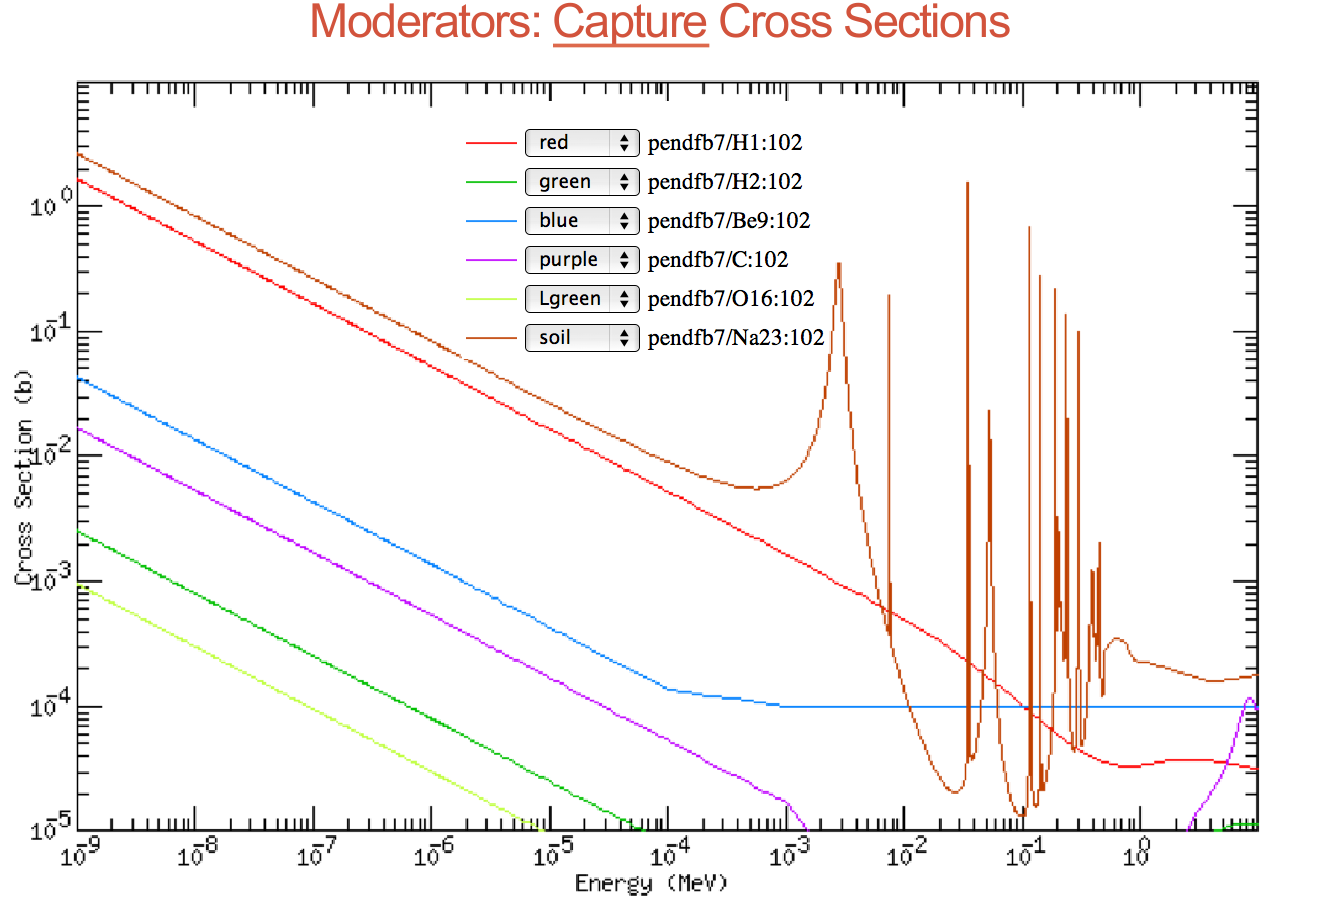
\includegraphics[width=4in]{images/capture-xs.png}
  \\
  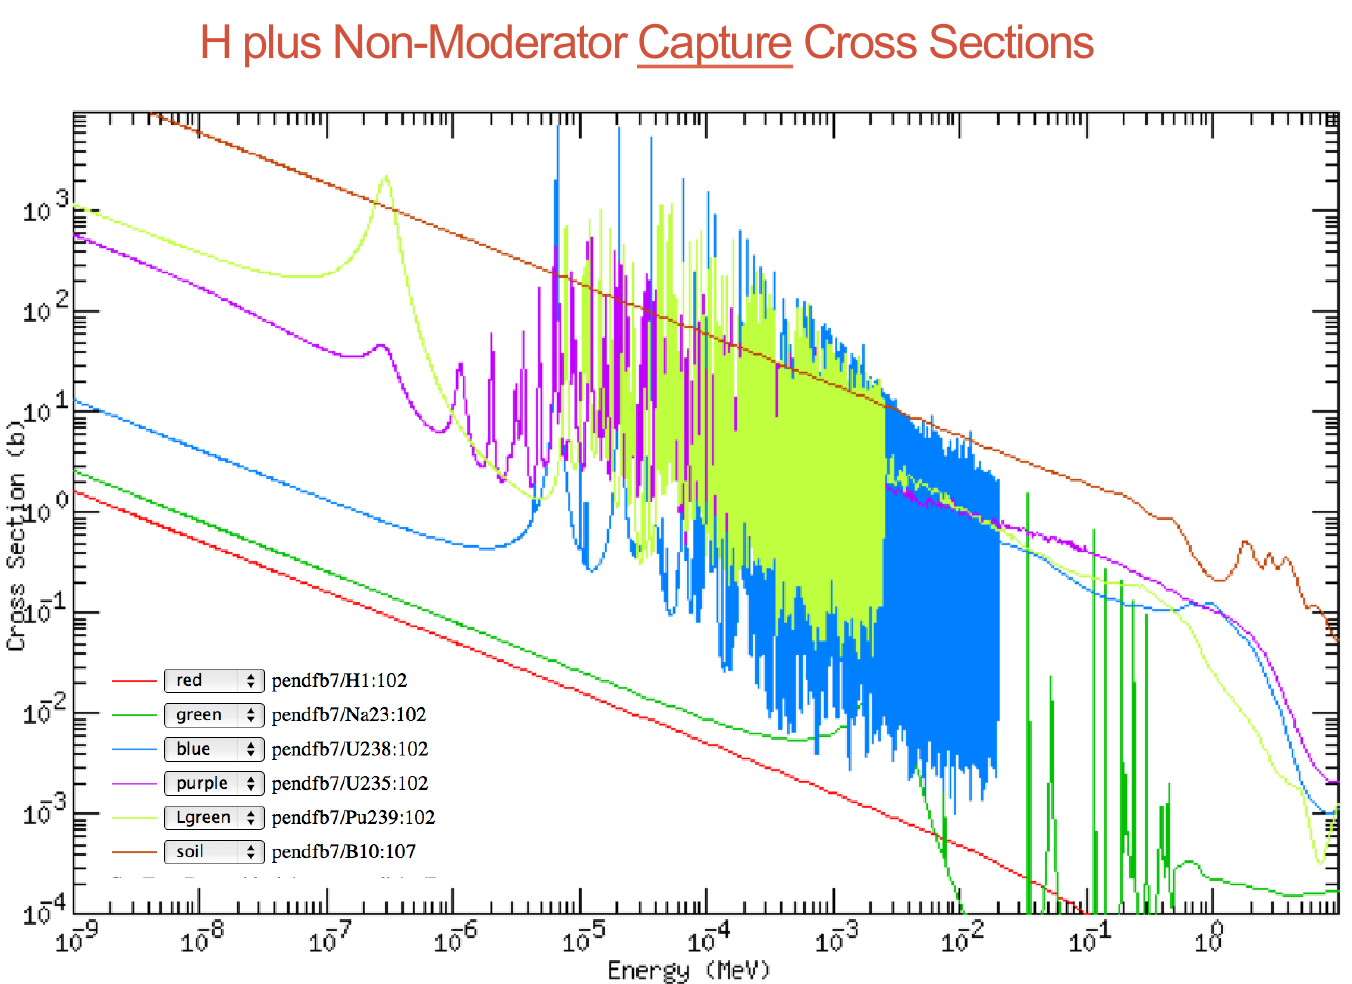
\includegraphics[width=4in]{images/capture-xs-2.png}
  \caption{Capture Cross Section} \label{capture-xs}
\end{figure}
\begin{enumerate}
\item H has no resonance; it has the highest scattering xs in LWR, so we can ignore any other isotopic's neutron scattering.   
\item Na has a huge resonance in 23 keV, and more resonances at higher energies because it is a heavy isotope.
\item Near zero energy,
\eqn{ \sigma(E\to 0) = }
\item Resonance at 6 to 7 eV: U238. 
\item U235's thermal elastic xs is larger than 238's, and they both have resonance around the same range.   
\item A small resonance at .3 eV: Pu239 (its signiture is a super low energy scattering xs). 
\end{enumerate}

\item Given an unknown material type, all we care is to count the nucleus density of each material and look at it's xs. 
\item Average fission neutron energy: 2 MeV; average peak fission energy: 1 MeV; see fission sepctrum. 

\item Core decay heat after 1 day is about 1\% rated. 


\end{enumerate}
%%%%%%%%%%%%%%%%%%%%%%%%% Qualify Exam End %%%%%%%%%%%%%%%%%%%%%%%%%%%%



\end{document}
